\documentclass[a4paper,10.5pt,oneside]{report}

\usepackage[utf8]{inputenc}
\usepackage[T1]{fontenc}
\usepackage[margin=2.1cm]{geometry}
\usepackage{amsmath,amssymb}
\usepackage{graphicx}
\usepackage{booktabs}
\usepackage{float}
\usepackage{caption}
\usepackage{setspace}
\usepackage{tikz}
\usetikzlibrary{arrows.meta,positioning,calc}
\usepackage[round,authoryear]{natbib}
\usepackage[hidelinks]{hyperref}
\usepackage{bookmark}
\usepackage[titletoc]{appendix}

\graphicspath{{figures/}{./}}

\hypersetup{
    pdftitle={Estimating Respiratory Rate from ECG Data},
    pdfauthor={Guangmei Tang},
    bookmarksopen=true,
    bookmarksnumbered=true
}

\setcounter{tocdepth}{1}
\setcounter{secnumdepth}{1}
\setlength{\parindent}{0pt}
\setlength{\parskip}{0.45em}
\setstretch{1.05}

\begin{document}

\begin{titlepage}
\begin{center}

% University banner
\includegraphics[width=0.35\textwidth]{figures/uom_banner.pdf}\\[0.3cm]

\textsc{\Large Final Report}\\[0.3cm]

% Title
\HRule \\[0.3cm]

{\huge \bfseries
The Art of Scientific Computing:\\[0.2cm]
Respiratory Rates: Determining breathing rates through\\
electrocardiogram data analysis
}\\[0.3cm]

\HRule \\[0.8cm]

% Author and subject code
\begin{minipage}{0.45\textwidth}
\begin{flushleft} \large
\textit{Author:}\\
Guangmei Tang\\[0.2cm]
\textit{Student ID:}\\
1562065
\end{flushleft}
\end{minipage}
\begin{minipage}{0.45\textwidth}
\begin{flushright} \large
\textit{Subject Code:}\\
COMP90072
\end{flushright}
\end{minipage}

\vfill

% Faculty and university
Faculty of Science\\
The University of Melbourne
\\[0.7cm]

% Submission date
{\small Submission Date: October 2026}
\\[1.2cm]

% Subject coordinator
Subject Coordinator: A/Prof Suzie Sheehy
\\[0.8cm]

\end{center}
\end{titlepage}

\pagenumbering{roman}

\chapter*{Summary}
\addcontentsline{toc}{chapter}{Summary}

This report investigates whether respiratory-related information can be estimated from long-duration electrocardiogram (ECG) recordings. PhysioNet Apnea-ECG record \texttt{a01}, sampled at 100 Hz over approximately 8.21 hours, was used to develop a reproducible Python workflow. The supplied QRS annotations were used to calculate 29,937 R--R intervals. These intervals were checked for clearly unrealistic values, interpolated to a regular 4 Hz grid, detrended, and analysed using Welch's power spectral density method within the 0.15--0.40 Hz frequency range.

The first five-minute window produced an estimated respiratory-related rate of 9.4 breaths/min. Across 98 complete five-minute windows, the estimates ranged from 9.38 to 19.69 breaths/min, with a mean of 13.58 breaths/min, showing that the selected spectral component changed over time. The analysis therefore shows that a reproducible respiratory-related frequency estimate can be extracted from the R--R interval series. However, the estimates were not directly compared with a respiratory reference signal, so they should be interpreted as ECG-derived respiratory-related estimates rather than validated measurements of breathing rate.

\clearpage
\tableofcontents
\clearpage
\pagenumbering{arabic}

\chapter{Introduction}

\section{Background and Motivation}

Respiratory rate is an important physiological measurement, but direct measurement usually requires either manual counting or a dedicated respiratory sensor. An alternative is to estimate breathing-related information from signals that are already being recorded. The electrocardiogram (ECG) is such a kind of signal. A review by \citet{charlton2018} shows that breathing rate can be estimated from ECG-derived signals using several approaches.

The physiological motivation for this project is respiratory sinus arrhythmia (RSA). Breathing can regulate heart rate, causing the interval between successive heartbeats to shorten and lengthen with respiration. Methods based on this effect have been used to estimate breathing rate from heart-rate variability \citep{schaefer2008}. This motivates analysing the timing between R peaks rather than trying to identify breathing directly from every detail of the ECG waveform.

Figure~\ref{fig:ecg_rsa_concept} illustrates how ECG R--R intervals are related to respiratory modulation. The QRS complex contains the R peak, and the time between two successive R peaks defines an R--R interval. During respiratory sinus arrhythmia, breathing can cause small cyclic changes in heart rate and therefore in the R--R interval.

\begin{figure}[H]
\centering

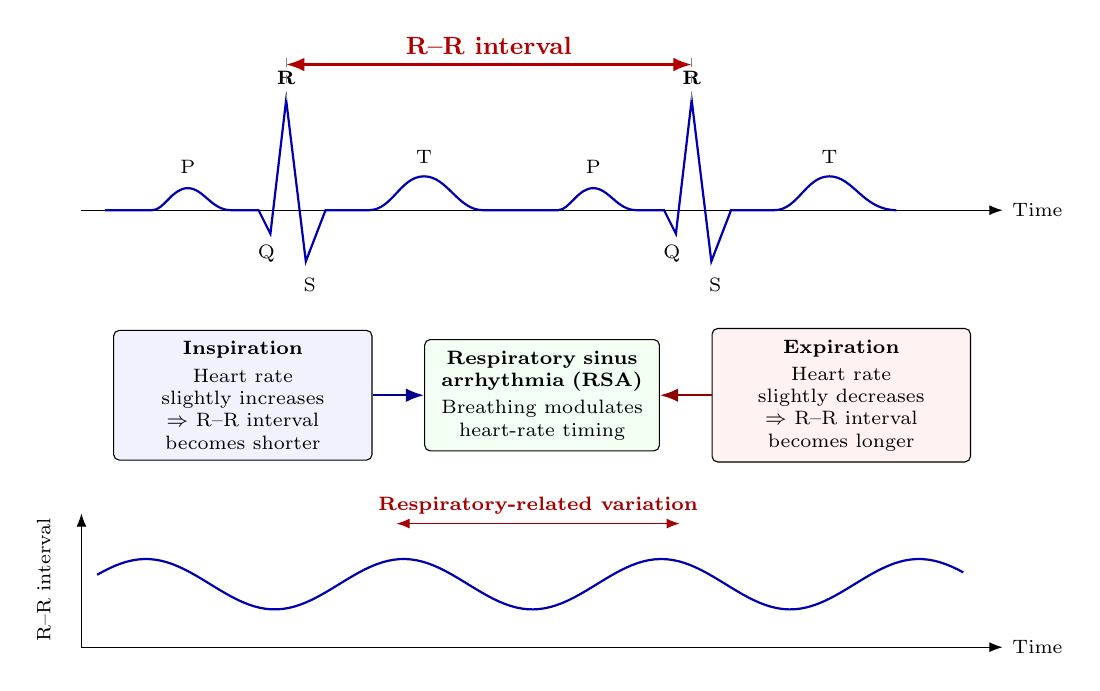
\begin{tikzpicture}[
    >=Latex,
    every node/.style={font=\scriptsize},
    sidebox/.style={
        draw,
        rounded corners=2pt,
        align=center,
        text width=3.0cm,
        minimum height=1.35cm,
        inner sep=4pt
    },
    centerbox/.style={
        draw,
        rounded corners=2pt,
        align=center,
        text width=2.7cm,
        minimum height=1.35cm,
        inner sep=4pt
    }
]

% =========================================================
% 1. ECG waveform
% =========================================================

\draw[->] (0,5.0) -- (11.7,5.0)
    node[right] {\scriptsize Time};

\draw[thick, blue!70!black]
(0.3,5.0) -- (0.9,5.0)
.. controls (1.05,5.0) and (1.15,5.28) .. (1.35,5.28)
.. controls (1.55,5.28) and (1.65,5.0) .. (1.9,5.0)
-- (2.25,5.0)
-- (2.40,4.70)
-- (2.60,6.40)
-- (2.85,4.35)
-- (3.10,5.0)
-- (3.65,5.0)
.. controls (3.95,5.0) and (4.05,5.43) .. (4.35,5.43)
.. controls (4.65,5.43) and (4.78,5.0) .. (5.10,5.0)

-- (6.05,5.0)
.. controls (6.20,5.0) and (6.30,5.28) .. (6.50,5.28)
.. controls (6.70,5.28) and (6.80,5.0) .. (7.05,5.0)
-- (7.40,5.0)
-- (7.55,4.70)
-- (7.75,6.40)
-- (8.00,4.35)
-- (8.25,5.0)
-- (8.80,5.0)
.. controls (9.10,5.0) and (9.20,5.43) .. (9.50,5.43)
.. controls (9.80,5.43) and (9.93,5.0) .. (10.35,5.0);

% ECG labels
\node at (1.35,5.55) {P};
\node at (2.35,4.45) {Q};
\node at (2.60,6.68) {\textbf{R}};
\node at (2.90,4.05) {S};
\node at (4.35,5.68) {T};

\node at (6.50,5.55) {P};
\node at (7.50,4.45) {Q};
\node at (7.75,6.68) {\textbf{R}};
\node at (8.05,4.05) {S};
\node at (9.50,5.68) {T};

% R-R interval
\draw[dashed, gray] (2.60,6.40) -- (2.60,7.02);
\draw[dashed, gray] (7.75,6.40) -- (7.75,7.02);

\draw[<->, thick, red!70!black]
(2.60,6.85) --
node[above, font=\small\bfseries] {R--R interval}
(7.75,6.85);


% =========================================================
% 2. Respiration effect: three boxes on ONE row
% =========================================================

\node[
    sidebox,
    fill=blue!5
] (insp) at (2.05,2.65)
{
\textbf{Inspiration}\\[2pt]
Heart rate slightly increases\\
$\Rightarrow$ R--R interval becomes shorter
};

\node[
    centerbox,
    fill=green!5
] (rsa) at (5.85,2.65)
{
\textbf{Respiratory sinus}\\
\textbf{arrhythmia (RSA)}\\[2pt]
Breathing modulates\\
heart-rate timing
};

\node[
    sidebox,
    fill=red!5
] (exp) at (9.65,2.65)
{
\textbf{Expiration}\\[2pt]
Heart rate slightly decreases\\
$\Rightarrow$ R--R interval becomes longer
};

% arrows between boxes
\draw[->, thick, blue!55!black]
(insp.east) -- (rsa.west);

\draw[<-, thick, red!55!black]
(rsa.east) -- (exp.west);


% =========================================================
% 3. R-R interval variation
% =========================================================

\draw[->] (0,-0.55) -- (11.7,-0.55)
    node[right] {\scriptsize Time};

\draw[->] (0,-0.55) -- (0,1.15);

\node[rotate=90] at (-0.48,0.30)
{R--R interval};

% sinusoidal R-R variation
\draw[
    thick,
    blue!70!black,
    domain=0.2:11.2,
    samples=150
]
plot (
    \x,
    {0.25 + 0.32*sin(110*\x)}
);

% respiratory-related variation label
\draw[<->, red!65!black]
(4.0,1.02) -- (7.6,1.02);

\node[
    above,
    font=\scriptsize\bfseries,
    text=red!65!black
] at (5.80,1.02)
{Respiratory-related variation};

\end{tikzpicture}

\caption{Conceptual relationship between ECG R--R intervals and respiratory
modulation. During respiratory sinus arrhythmia, inspiration and expiration
produce small cyclic changes in heart rate and therefore in the R--R interval.
These variations can contain respiratory-related information.}

\label{fig:ecg_rsa_concept}

\end{figure}

R--R timing is useful, but it is not affected by respiration alone. Normal heart-rate variability, ectopic beats, measurement artefacts and other physiological processes can also change the interval sequence. This is why the final estimate is described as \emph{respiratory-related} rather than as a direct respiratory measurement.

\section{Data, Aim and Research Questions}

The data are taken from the PhysioNet Apnea-ECG Database \citep{penzel2000}.
PhysioNet provides open physiological datasets and tools for reproducible
signal analysis \citep{goldberger2000}. The present report focuses on record
\texttt{a01}, a long single-channel ECG sampled at 100 Hz. The record contains
2,957,000 samples, corresponding to approximately 8.21 hours.

Four WFDB files are used in the analysis: \texttt{a01.dat} contains the ECG
waveform, \texttt{a01.hea} contains sampling and scaling metadata,
\texttt{a01.qrs} contains supplied QRS annotations, and \texttt{a01.apn}
contains minute-level apnea labels. The annotations are used as references
rather than assumed to be perfect ground truth.

The central aim is to determine whether the R--R interval time series can be
used to obtain a reproducible respiratory-related frequency estimate from ECG
alone. The work is organised around four questions:

\begin{enumerate}
    \item Can the available QRS timing information be used reliably to
    construct a long R--R interval time series?
    \item Can periodic variation in the R--R series be converted into a
    meaningful respiratory-related frequency estimate?
    \item How stable is that estimate when the recording is divided into
    different time windows?
    \item Do the ECG-derived respiratory features differ between normal and
    apnea-labelled minutes?
\end{enumerate}

The initial project plan also proposed developing an independent R-peak
detector and comparing several records. During implementation, the supplied QRS
annotations were found to align well with visible R peaks in the inspected
segments. The final scope was therefore narrowed so that more attention could
be given to the respiratory-rate pipeline, parameter choices, time variation,
and limitations. This choice was made to keep the project focused, while QRS detection is still considered an important part of ECG analysis. The optional apnea classifier is retained
only as a small extension after the core analysis is complete.

\chapter{Data and Preliminary Analysis}

\section{Data Integrity and Direct Waveform Exploration}

The ECG data are stored as 16-bit integer values and are converted to millivolts using the gain given in the header file. For record a01, the gain is 200 digital units per mV, with a baseline value of zero, so

\begin{equation}
    x_{\mathrm{mV}}
    =
    \frac{x_{\mathrm{digital}}-x_{\mathrm{zero}}}{\mathrm{gain}}.
    \label{eq:scaling}
\end{equation}

The header reports 2,957,000 samples. Because the waveform is stored as
16-bit values, the expected data size is $2\times2{,}957{,}000=5{,}914{,}000$
bytes. Before analysis, the number of ECG samples was checked against the value recorded in the header file. This ensured that the data file had been downloaded completely and that the full recording was available for analysis.

Before using any R-peak locations, the waveform itself was explored. This is
useful because it describes signal amplitude and large-scale variability
without depending on the QRS annotations. Table~\ref{tab:waveformsummary}
summarises the whole record and the first 10 seconds.

\begin{table}[H]
\centering
\caption{Direct waveform summary for record \texttt{a01}. The statistics are
calculated from ECG samples before R--R interval processing.}
\label{tab:waveformsummary}
\begin{tabular}{lrr}
\toprule
Quantity & Whole record & First 10 s \\
\midrule
Minimum amplitude (mV) & -1.655 & -0.825 \\
Maximum amplitude (mV) &  2.440 &  1.720 \\
Mean amplitude (mV)    &  0.0006 & -0.0001 \\
Standard deviation (mV)&  0.244 &  0.255 \\
\bottomrule
\end{tabular}
\end{table}

The full recording has a wider amplitude range than the first 10 seconds, showing that more extreme ECG amplitudes occur elsewhere in the recording. However, this simple comparison cannot determine whether these values are caused by normal waveform variation, unusual beats, or short artefacts. The whole-record mean remains close to zero, suggesting that there is no large overall shift in the ECG baseline.

To check whether the overall signal variability changes gradually over the
night, the ECG was divided into consecutive 30-minute blocks and the standard
deviation of each block was calculated. Figure~\ref{fig:ecgstd} shows that the
30-minute standard deviations remain in a relatively narrow range of
approximately 0.235--0.256 mV. The block means are also close to zero
(approximately 0.0003--0.0010 mV). The result does not mean that there are no short artefacts or unusual beats, but the overall ECG amplitude appears to remain fairly stable throughout the recording.

\begin{figure}[H]
    \centering
    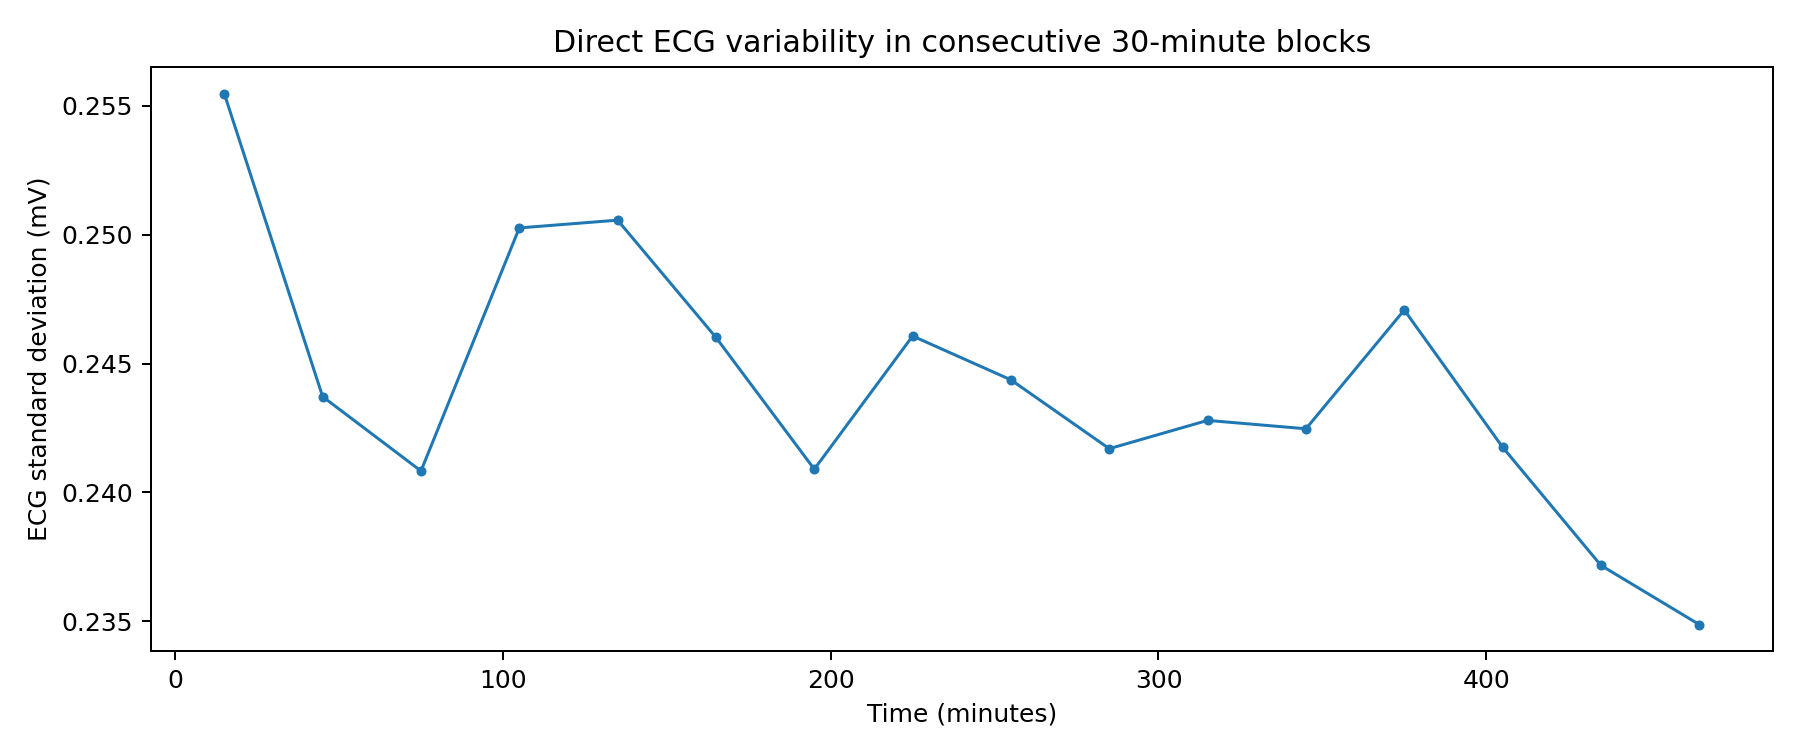
\includegraphics[width=0.84\linewidth]{ecg_std_30min_blocks.png}
    \caption{Standard deviation of the raw ECG in consecutive 30-minute blocks.
    The overall variability changes only modestly, although short local
    artefacts may still occur within each block.}
    \label{fig:ecgstd}
\end{figure}

Only record \texttt{a01} is explored in this level of detail, so these waveform
properties should not be assumed to be identical for every subject in the
database.

\section{ECG Morphology and Annotation Alignment}

Figure~\ref{fig:ecgfirst} shows the first 10 seconds of the recording. Repeated
sharp R peaks are clearly visible. The waveform is qualitatively consistent
with the P--QRS--T structure introduced in Figure~\ref{fig:ecg_rsa_concept}, but the
peak amplitudes are not identical from beat to beat and the real signal is less
regular than an ideal schematic.

No large noise or baseline disturbance is obvious in this short segment, although a 10-second visual inspection cannot represent the signal quality of the full recording.

\begin{figure}[H]
    \centering
    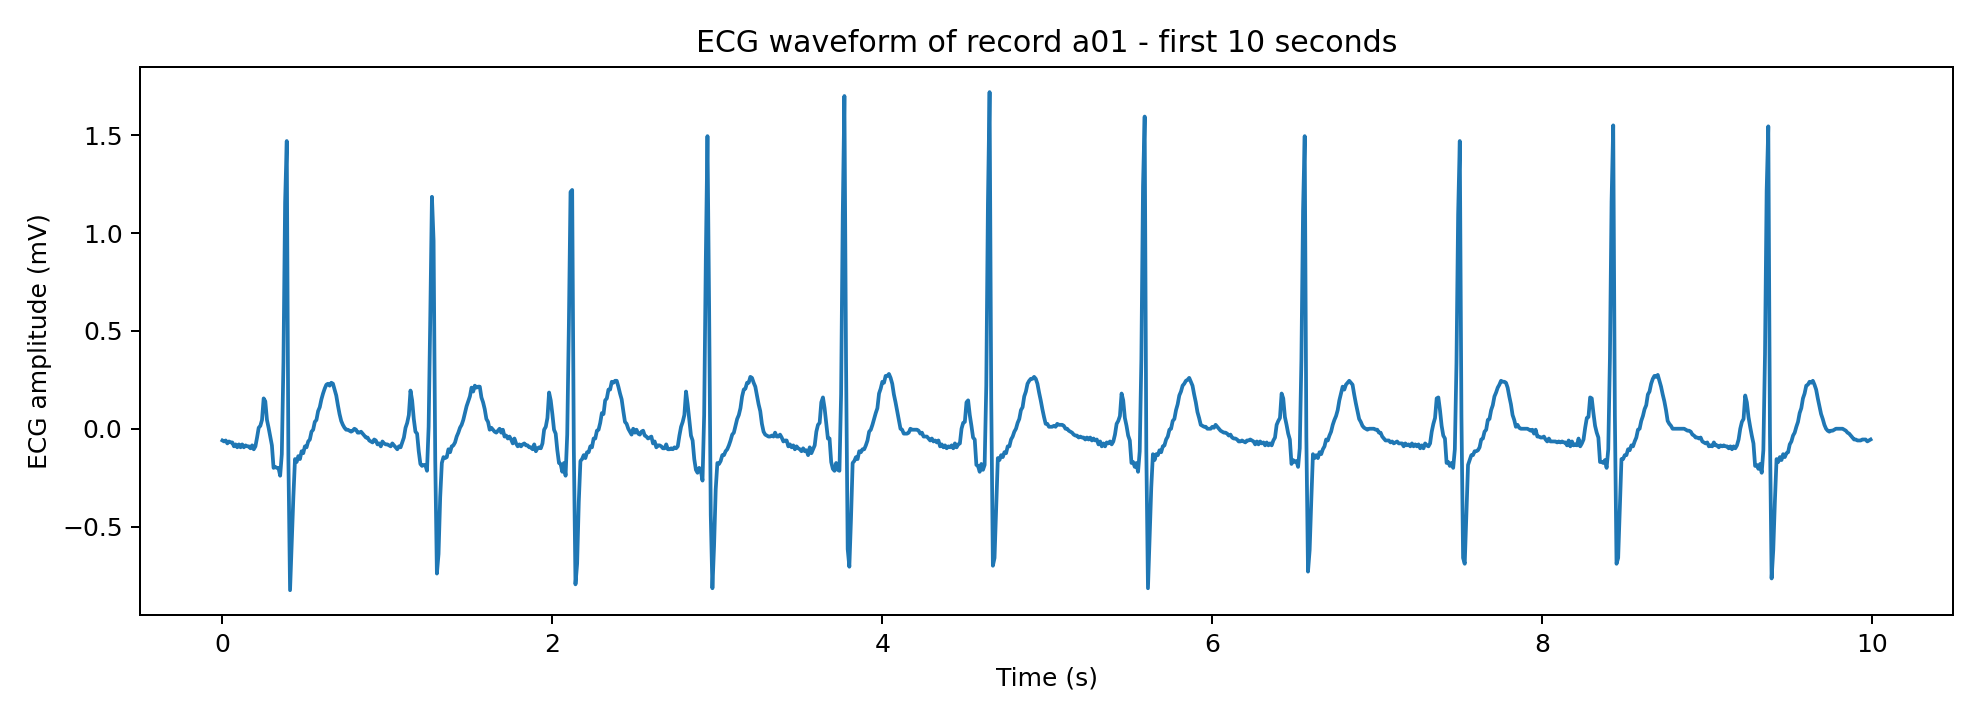
\includegraphics[width=0.88\linewidth]{ecg_first10s.png}
    \caption{First 10 seconds of record \texttt{a01}. Repeated QRS complexes are
    visible, while the R-peak amplitude varies between beats.}
    \label{fig:ecgfirst}
\end{figure}

The supplied QRS annotations were converted from sample numbers to time and plotted together with the ECG signal. As shown in Figure~\ref{fig:ecgqrs}, the annotation times generally line up well with the visible R peaks. This check
supports using the supplied annotations as the timing reference for the main
analysis. It does not prove that every annotation across 8.21 hours is correct;
QRS timing errors can affect downstream heart-rate-variability measures
\citep{weinstein2026}.

\begin{figure}[H]
    \centering
    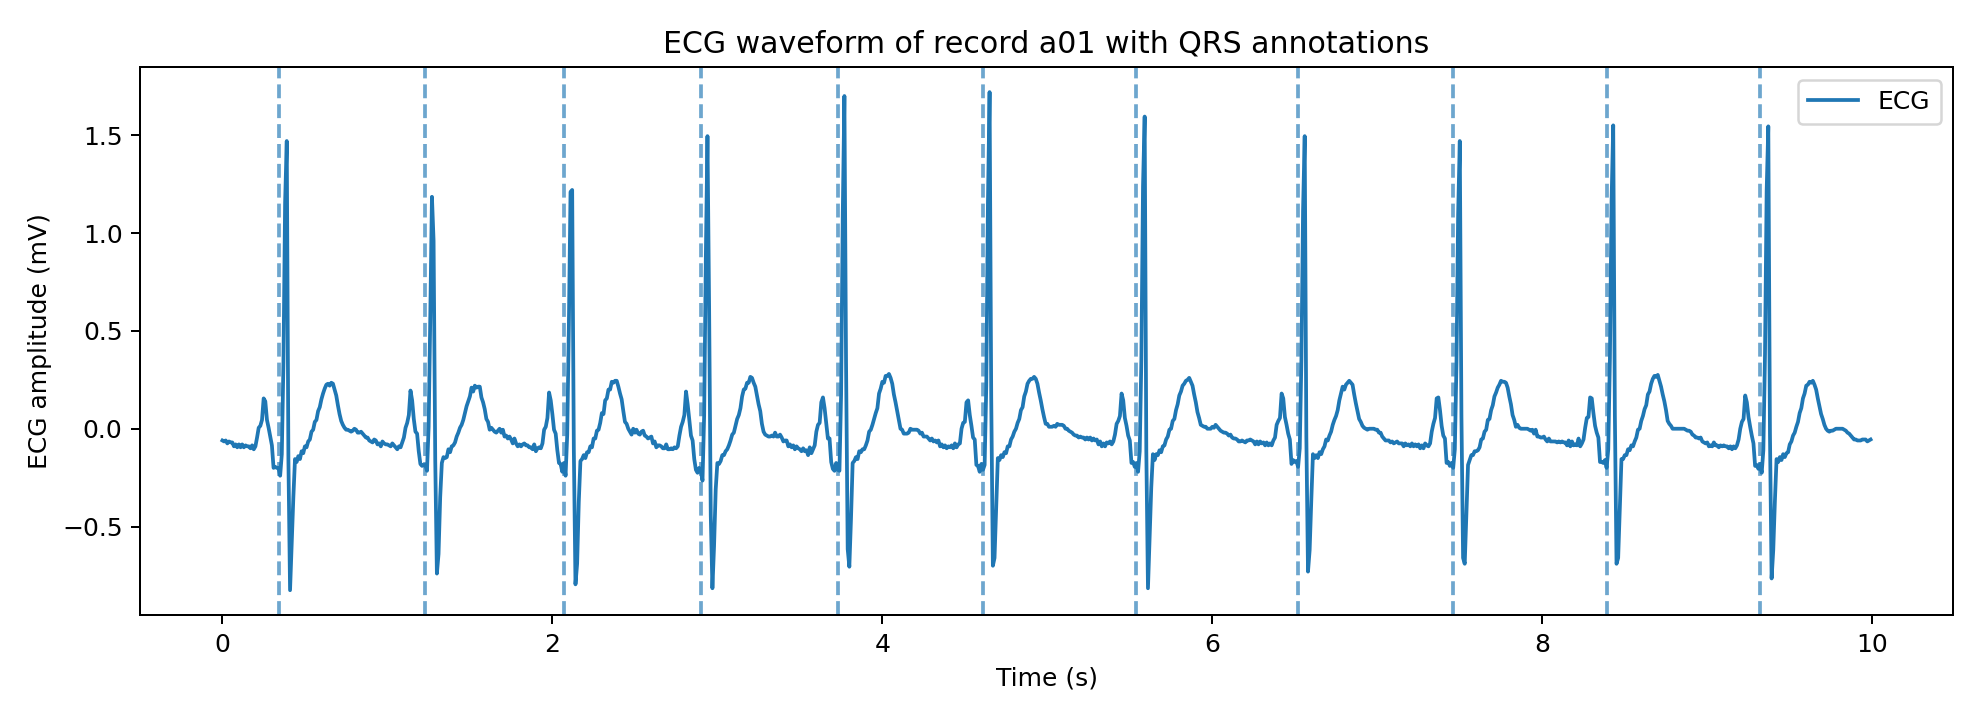
\includegraphics[width=0.88\linewidth]{ecg_qrs.png}
    \caption{ECG waveform with supplied QRS annotations. The dashed lines align
    closely with the R peaks in the inspected 10-second interval.}
    \label{fig:ecgqrs}
\end{figure}

The apnea annotations are minute-level labels. Record \texttt{a01} contains
489 labelled minutes, of which 470 are labelled \texttt{A} and 19 are labelled
\texttt{N}. Figure~\ref{fig:ecgapnea} shows one apnea-labelled minute together
with ECG and QRS timing. The plot is visually dense because many heartbeats
occur within 60 seconds, but it confirms that ECG, QRS and apnea annotations
share the same time axis.

\begin{figure}[H]
    \centering
    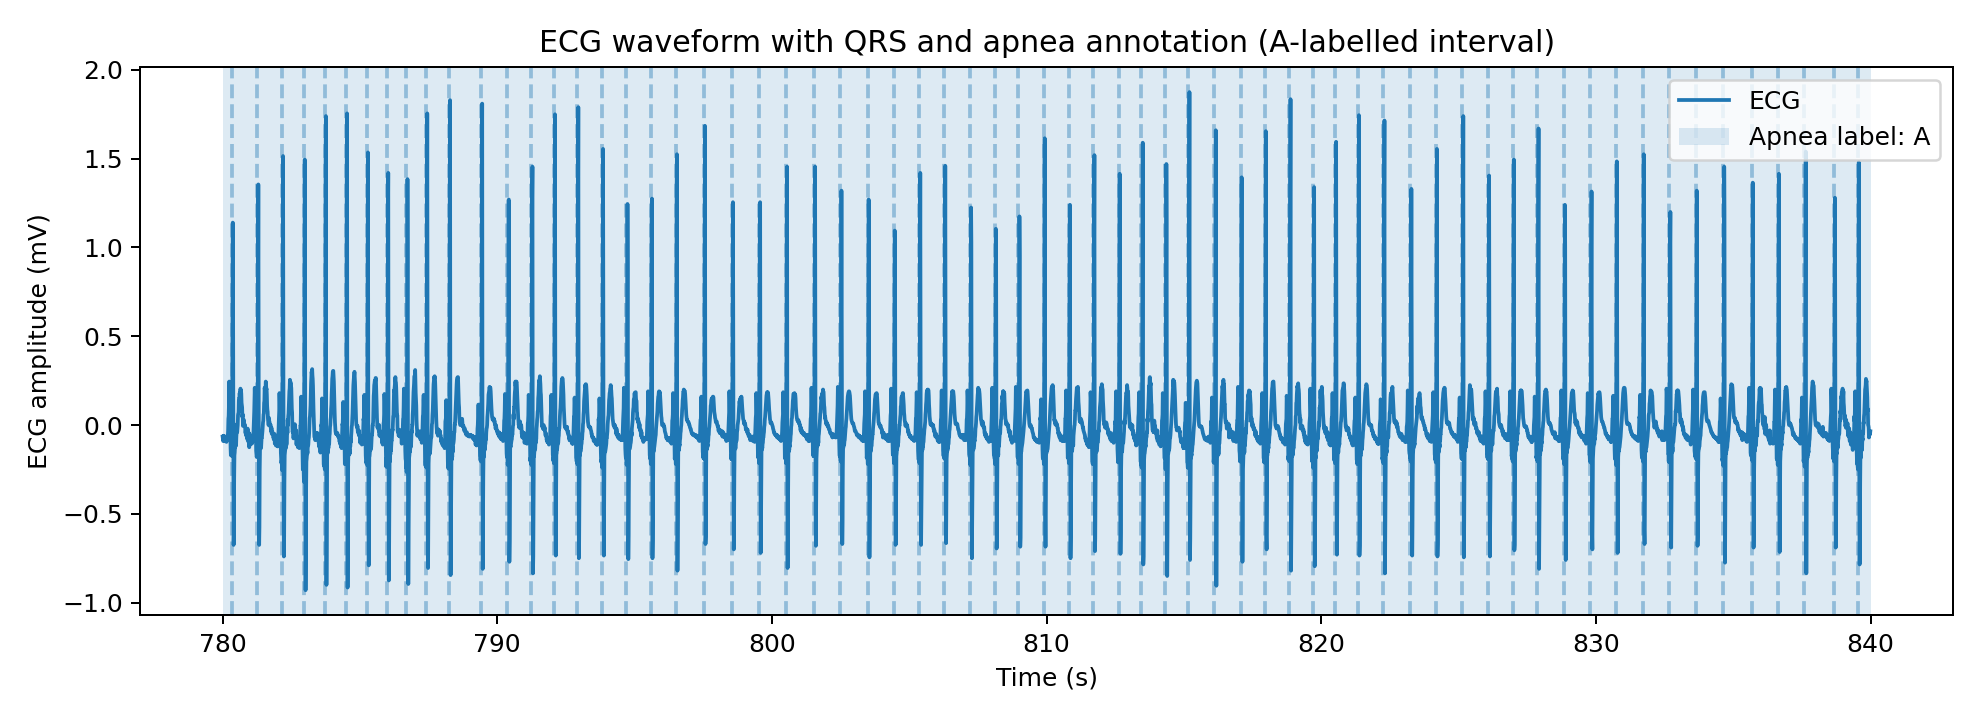
\includegraphics[width=0.88\linewidth]{ecg_qrs_apnea_window.png}
    \caption{ECG waveform and QRS annotations during one apnea-labelled
    60-second interval. The shaded region represents the apnea label.}
    \label{fig:ecgapnea}
\end{figure}

\chapter{Methodology}

Figure~\ref{fig:pipeline} shows the core processing pipeline. This method is designed to maintain interpretability: each step can be checked independently before proceeding to the next step.

\begin{figure}[H]
\centering
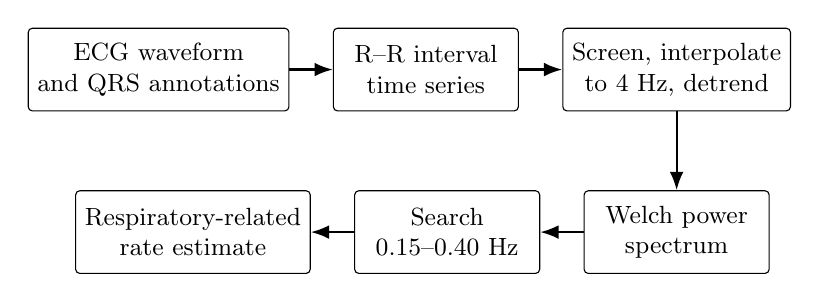
\begin{tikzpicture}[
    node distance=0.75cm and 0.55cm,
    box/.style={draw, rounded corners=1.5pt, align=center, minimum height=1.05cm,
    minimum width=2.35cm, font=\small},
    arr/.style={-Latex, thick}
]
\node[box] (ecg) {ECG waveform\\and QRS annotations};
\node[box, right=of ecg] (rr) {R--R interval\\time series};
\node[box, right=of rr] (reg) {Screen, interpolate\\to 4 Hz, detrend};
\node[box, below=1.0cm of reg] (psd) {Welch power\\spectrum};
\node[box, left=of psd] (band) {Search\\0.15--0.40 Hz};
\node[box, left=of band] (rate) {Respiratory-related\\rate estimate};
\draw[arr] (ecg) -- (rr);
\draw[arr] (rr) -- (reg);
\draw[arr] (reg) -- (psd);
\draw[arr] (psd) -- (band);
\draw[arr] (band) -- (rate);
\end{tikzpicture}
\caption{Core analysis pipeline from ECG/QRS timing to an ECG-derived
respiratory-rate estimate.}
\label{fig:pipeline}
\end{figure}

\section{R--R Time Series and Preprocessing}

If consecutive QRS annotations occur at sample indices $n_i$ and $n_{i+1}$,
their times are $t_i=n_i/f_s$, where $f_s=100$ Hz. The R--R interval is

\begin{equation}
    RR_i=t_{i+1}-t_i,
    \label{eq:rr}
\end{equation}

and is assigned to the midpoint

\begin{equation}
    t_{RR,i}=\frac{t_i+t_{i+1}}{2}.
    \label{eq:rrtime}
\end{equation}

Record \texttt{a01} contains 29,938 QRS annotations and therefore 29,937
consecutive R--R intervals.

The R--R sequence is irregularly sampled because each value is tied to a heartbeat rather than to a fixed time interval. Standard FFT-based spectral
methods assume samples on a regular time grid, so a preprocessing stage is
needed before frequency analysis. R--R intervals shorter than 0.30 s or longer than 2.00 s are treated as unrealistic and removed from the analysis. This range is roughly equivalent to 30--200 beats/min and is only used to remove clearly unrealistic values, not to define a clinically normal heart rate.

After screening, the R--R series is linearly interpolated to 4 Hz and linearly
detrended. The 4 Hz grid has a Nyquist frequency of

\begin{equation}
    f_N=\frac{4}{2}=2~\mathrm{Hz},
\end{equation}

which is much higher than the respiratory band used later. Therefore, the
regularised sampling rate is sufficient for the spectral range of interest.

\section{Respiratory-Rate Estimation and Parameter Choices}

The processed R--R series is analysed using Welch's power spectral density
estimate \citep{welch1967}. Welch's method divides a signal into shorter
segments, computes periodograms, and averages them. Compared with a single raw
periodogram, this reduces variance and gives a more stable description of the
frequency content within each analysis window.

The respiratory search band is

\[
0.15\leq f\leq0.40~\mathrm{Hz}.
\]

This is the conventional high-frequency range commonly used in
heart-rate-variability analysis and is strongly associated with respiratory
modulation \citep{taskforce1996}. It is used as a literature-supported search
range rather than as a claim that every possible breathing frequency lies
inside it.

For each time window, the largest power spectral density value inside the band
is selected. If the selected frequency is $f_r$ Hz, the ECG-derived
respiratory-rate estimate is

\begin{equation}
    R_{\mathrm{resp}}=60f_r
    \quad\text{breaths/min}.
    \label{eq:bpm}
\end{equation}

For sufficiently long windows, \texttt{nperseg}=256. At 4 Hz, the nominal
frequency spacing is

\begin{equation}
    \Delta f=\frac{4}{256}=0.015625~\mathrm{Hz},
\end{equation}

equivalent to 0.9375 breaths/min. This finite frequency resolution explains why
many five-minute estimates occur at repeated discrete values.

Table~\ref{tab:choices} collects the main analysis choices and the reason for
each one.

\begin{table}[H]
\centering
\caption{Main processing choices used in the ECG-to-respiratory pipeline.}
\label{tab:choices}
\begin{tabular}{p{0.28\linewidth} p{0.20\linewidth} p{0.43\linewidth}}
\toprule
Choice & Value & Reason \\
\midrule
ECG sampling rate & 100 Hz & Taken from the WFDB header; sufficient for timing the supplied QRS annotations. \\
R--R plausibility screen & 0.30--2.00 s & Removes only clearly implausible intervals; deliberately broad to avoid excessive editing. \\
Regular R--R grid & 4 Hz & Provides a uniform series for spectral analysis with Nyquist frequency well above the respiratory band. \\
Main analysis window & 5 min & Long enough to contain many respiratory cycles while still showing change over the night. \\
Respiratory search band & 0.15--0.40 Hz & Literature-supported HRV high-frequency band associated with respiratory modulation \citep{taskforce1996}. \\
Welch segment length & Up to 256 samples & Balances spectral averaging and frequency resolution for the regularised R--R series. \\
Apnea comparison window & 60 s & Matches the time scale of the supplied apnea annotations. \\
\bottomrule
\end{tabular}
\end{table}

A five-minute window is especially useful for the main estimator because even
at the lower band boundary, 0.15 Hz corresponds to about 9 cycles per minute,
or about 45 cycles within five minutes. In contrast, a 60-second window contains
far fewer cycles and therefore gives a coarser estimate. The one-minute
analysis is used only because the apnea labels themselves are minute-based. For five-minute windows, Welch analysis uses segments of up to 256 samples. For the one-minute analysis, the interpolated R--R series contains fewer than 256 samples, so the segment length is reduced to the available number of samples. As a result, the one-minute estimates have lower frequency resolution and less spectral averaging than the five-minute estimates.

\section{Robustness and Exploratory Extensions}

The estimator is first repeated over non-overlapping five-minute windows across
the full recording. This directly addresses whether the estimate is stable over
time rather than relying on one selected segment.

The same basic estimator is then applied to each labelled minute to compare
normal and apnea-labelled periods. Earlier studies have shown that sleep apnea
can be associated with characteristic changes in cardiac timing and
ECG-derived features \citep{penzel2002,dechazal2003}. The comparison in this
report is descriptive and exploratory.

A spectrogram is used as an additional time-frequency method. A spectrogram shows how the frequency content changes over time, rather than giving only one spectrum for the whole time window. Time-frequency analysis of
heart-period variability has previously been used in sleep-apnea studies
\citep{roche2003}.

Finally, a simple logistic-regression model is used as an optional extension.
Each minute is represented by the number of R--R intervals and the estimated
respiratory rate. For two features $x_1$ and $x_2$, the model has the form

\begin{equation}
P(A\mid x_1,x_2)
=
\frac{1}
{1+\exp[-(\beta_0+\beta_1x_1+\beta_2x_2)]}.
\label{eq:logistic}
\end{equation}

The data are split into 80\% for training and 20\% for testing, while keeping a similar proportion of normal and apnea-labelled samples in both sets. Before training, the two input features were scaled to a similar range. Since the number of samples labeled as apnea is far greater than the number of normal samples, class weights were also used to prevent the model from ignoring the smaller group of normal samples.
Short ECG epochs have been used in previous automated apnea studies
\citep{dechazal2004}, but the classifier here is not intended as a clinical
model.

\chapter{Results}

\section{Core R--R and Respiratory-Rate Results}

The first 10 R--R intervals are

\[
[0.89,\ 0.84,\ 0.83,\ 0.83,\ 0.88,\ 0.93,\ 0.98,\ 0.94,\ 0.93,\ 0.93]~\text{s}.
\]

Figure~\ref{fig:rr5} shows the first five minutes. The intervals vary mainly
between approximately 0.6 and 1.0 s. The R--R intervals do not change in a perfectly regular pattern. This is reasonable because they are affected by factors other than respiration.

\begin{figure}[H]
    \centering
    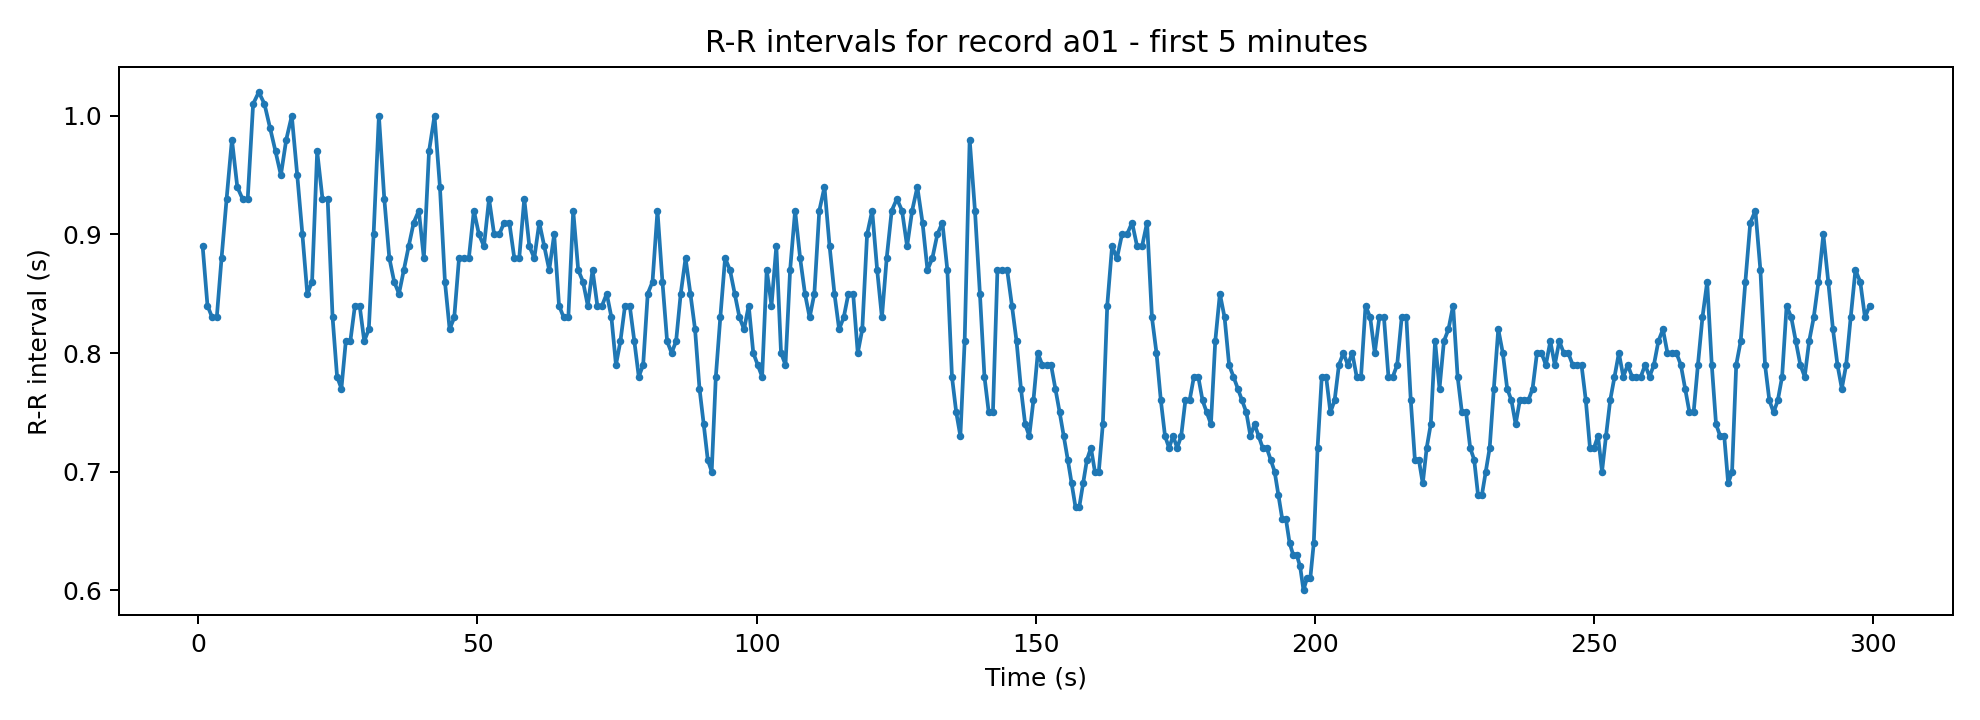
\includegraphics[width=0.90\linewidth]{rr_first5min.png}
    \caption{R--R intervals during the first five minutes of record
    \texttt{a01}. The variation is substantial enough to motivate a
    frequency-domain analysis, but it is not purely periodic.}
    \label{fig:rr5}
\end{figure}

All R--R intervals used in the five-minute and one-minute analyses were between 0.30 and 2.00 s. Therefore, this check did not remove any data and was only used to make sure that there were no clearly unrealistic values.

Figure~\ref{fig:rrinterp} compares the irregular R--R samples with the
regularised 4 Hz series. The interpolated curve follows the original samples
closely while providing a fixed time grid for spectral analysis.

\begin{figure}[H]
    \centering
    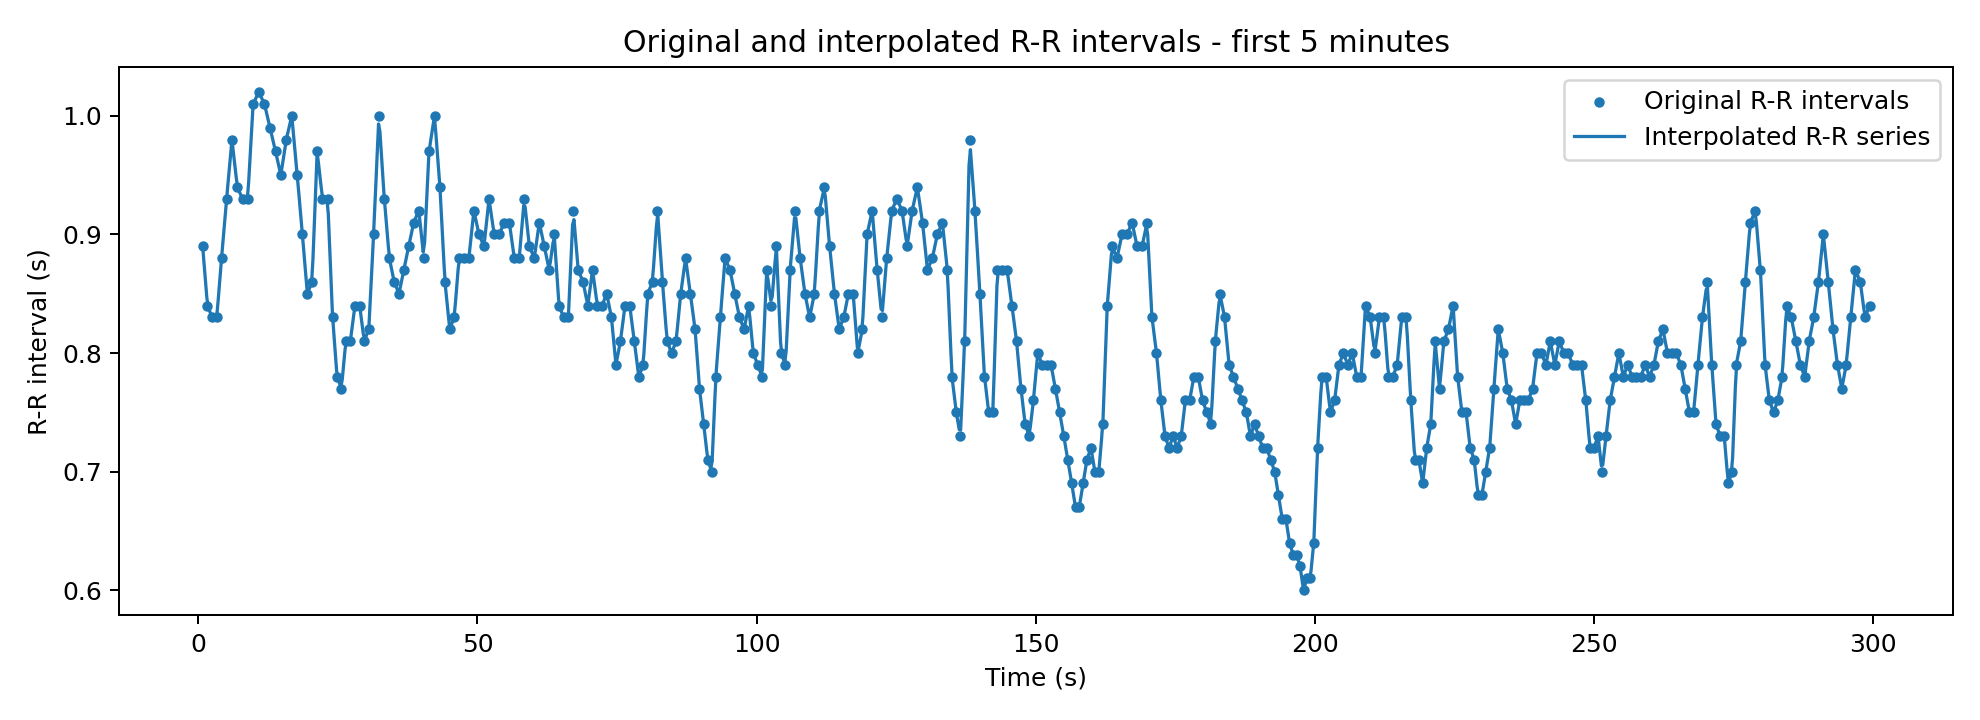
\includegraphics[width=0.90\linewidth]{rr_interpolation_first5min.png}
    \caption{Original and interpolated R--R intervals for the first five
    minutes. Interpolation regularises the time axis without visibly changing
    the main R--R pattern.}
    \label{fig:rrinterp}
\end{figure}

The first five-minute power spectrum is shown in
Figure~\ref{fig:spectrum5}. The largest component inside the 0.15--0.40 Hz
search band is 0.15625 Hz. Using Equation~\ref{eq:bpm},

\[
R_{\mathrm{resp}}
=
60(0.15625)
=
9.375
\approx 9.4~\text{breaths/min}.
\]

\begin{figure}[H]
    \centering
    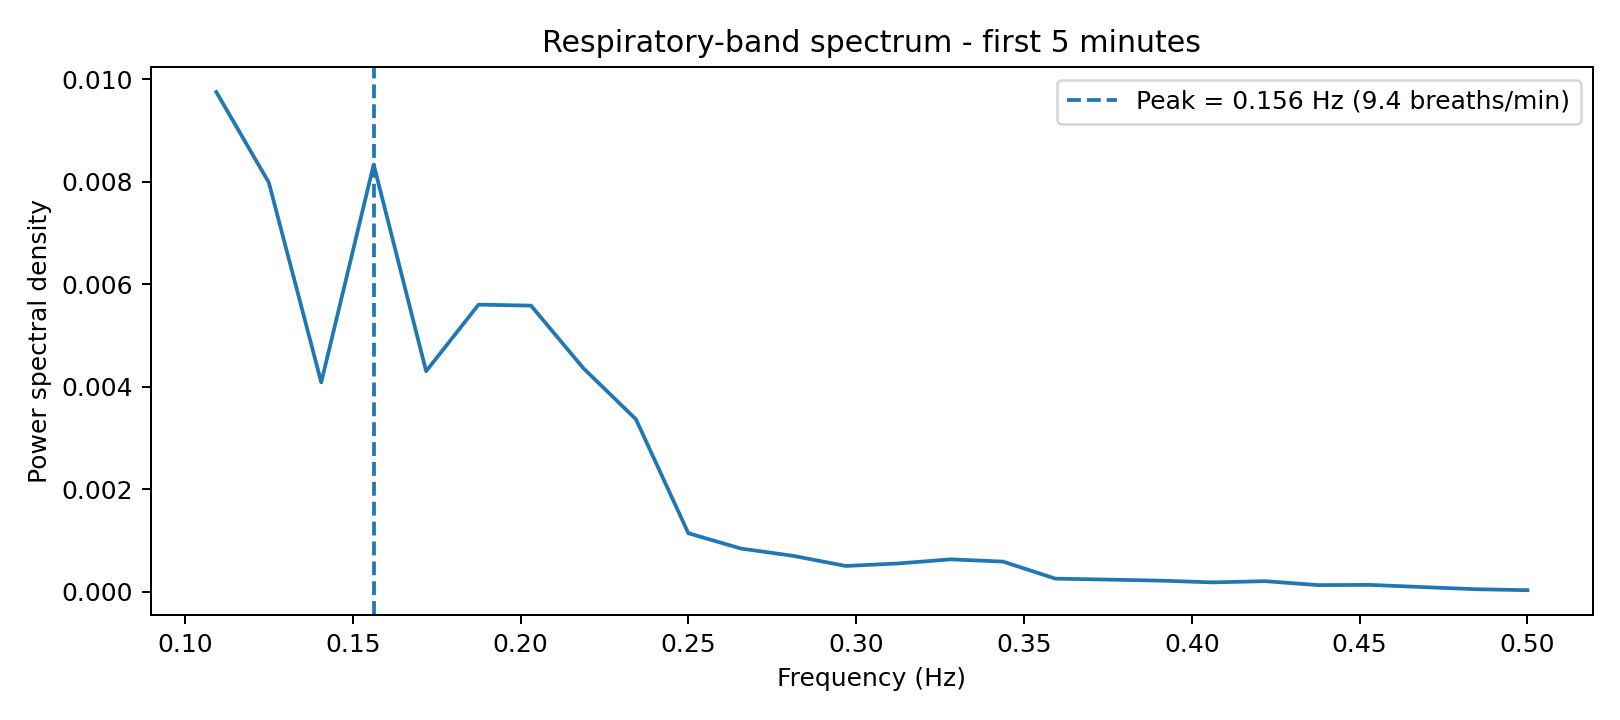
\includegraphics[width=0.86\linewidth]{respiratory_spectrum_first5min.png}
    \caption{Power spectrum of the processed R--R series for the first five
    minutes. The dashed line marks the selected in-band peak at 0.156 Hz
    (9.4 breaths/min). The wider 0.10--0.50 Hz range is displayed for context,
    while peak selection uses 0.15--0.40 Hz.}
    \label{fig:spectrum5}
\end{figure}

A strong low-frequency component is also visible below 0.15 Hz. This matters:
the value 9.4 breaths/min is the dominant component within the defined
search band, not a direct measurement of breathing.

\section{Stability Across the Recording}

The complete recording provides 98 non-overlapping five-minute windows. Only complete five-minute windows were included. The 98 windows cover the first 490 minutes of the recording, leaving the final 170 s outside this summary.
Table~\ref{tab:5minsummary} summarises the estimates.

\begin{table}[H]
\centering
\caption{Summary of five-minute ECG-derived respiratory-rate estimates for
record \texttt{a01}.}
\label{tab:5minsummary}
\begin{tabular}{lr}
\toprule
Statistic & Estimate (breaths/min) \\
\midrule
Number of windows & 98 \\
Minimum & 9.38 \\
Maximum & 19.69 \\
Mean & 13.58 \\
Median & 12.19 \\
Standard deviation & 4.08 \\
\bottomrule
\end{tabular}
\end{table}

The first five windows produce 9.38, 9.38, 14.06, 16.88 and
16.88 breaths/min. Figure~\ref{fig:windowtime} shows all 98 estimates over time
and makes the variability easier to see. The estimates do not remain near one
constant value; instead they repeatedly move between lower and higher parts of
the search band.

\begin{figure}[H]
    \centering
    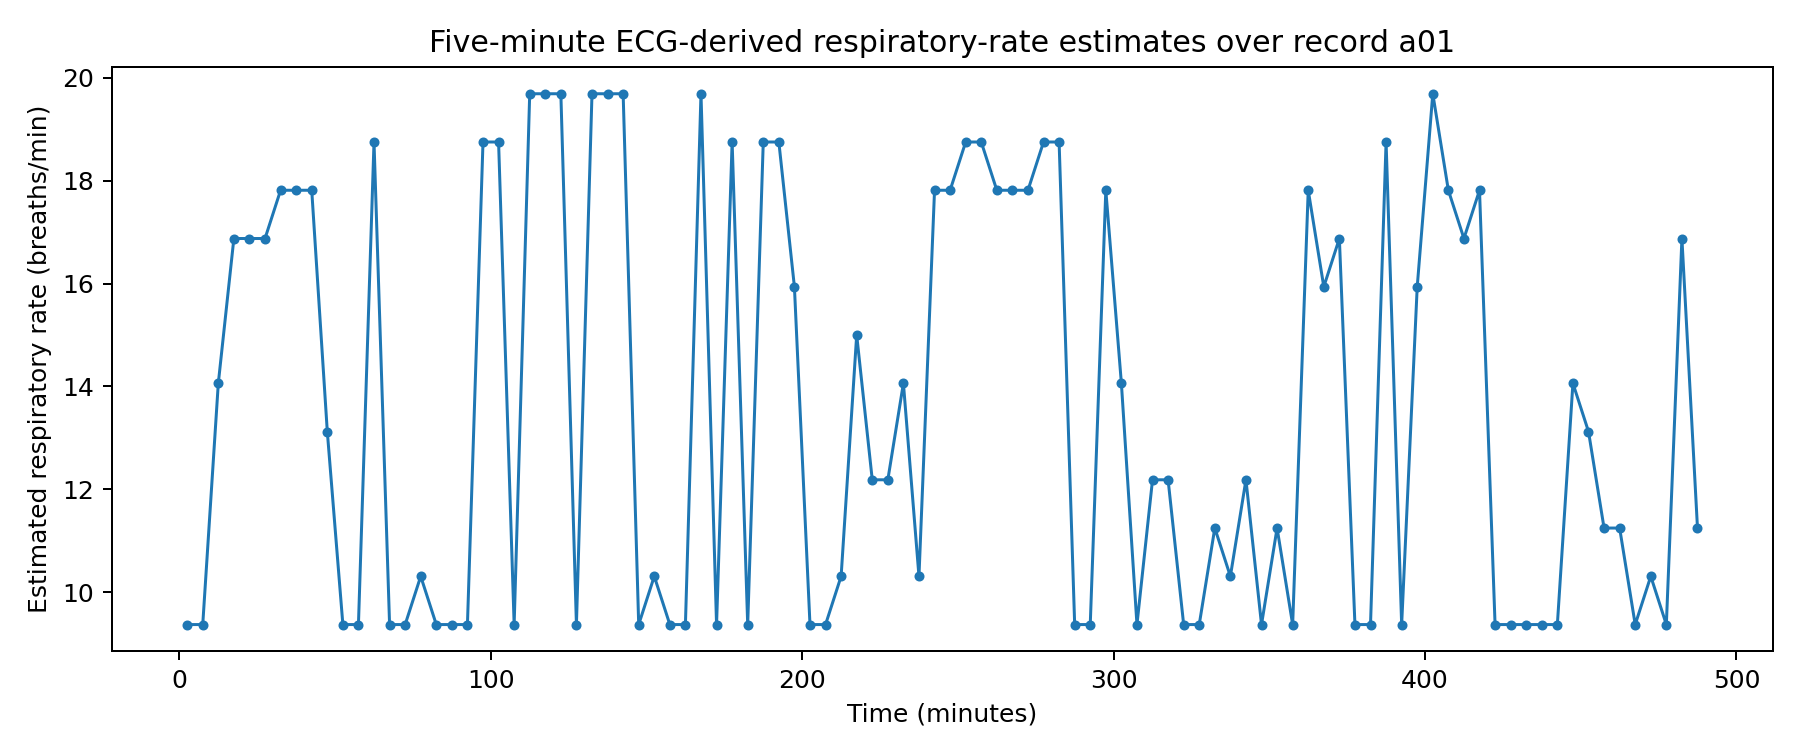
\includegraphics[width=0.90\linewidth]{respiratory_rate_5min_over_time.png}
    \caption{Five-minute ECG-derived respiratory-rate estimates across record
    \texttt{a01}. The variation over the night shows why a single short-window
    estimate is not representative of the full recording.}
    \label{fig:windowtime}
\end{figure}

The time-frequency view in Figure~\ref{fig:spectrogram} shows the same
conclusion. During the first 30 minutes, stronger spectral power occurs near
0.15--0.20 Hz in some intervals and around approximately 0.25--0.30 Hz in
others.

\begin{figure}[H]
    \centering
    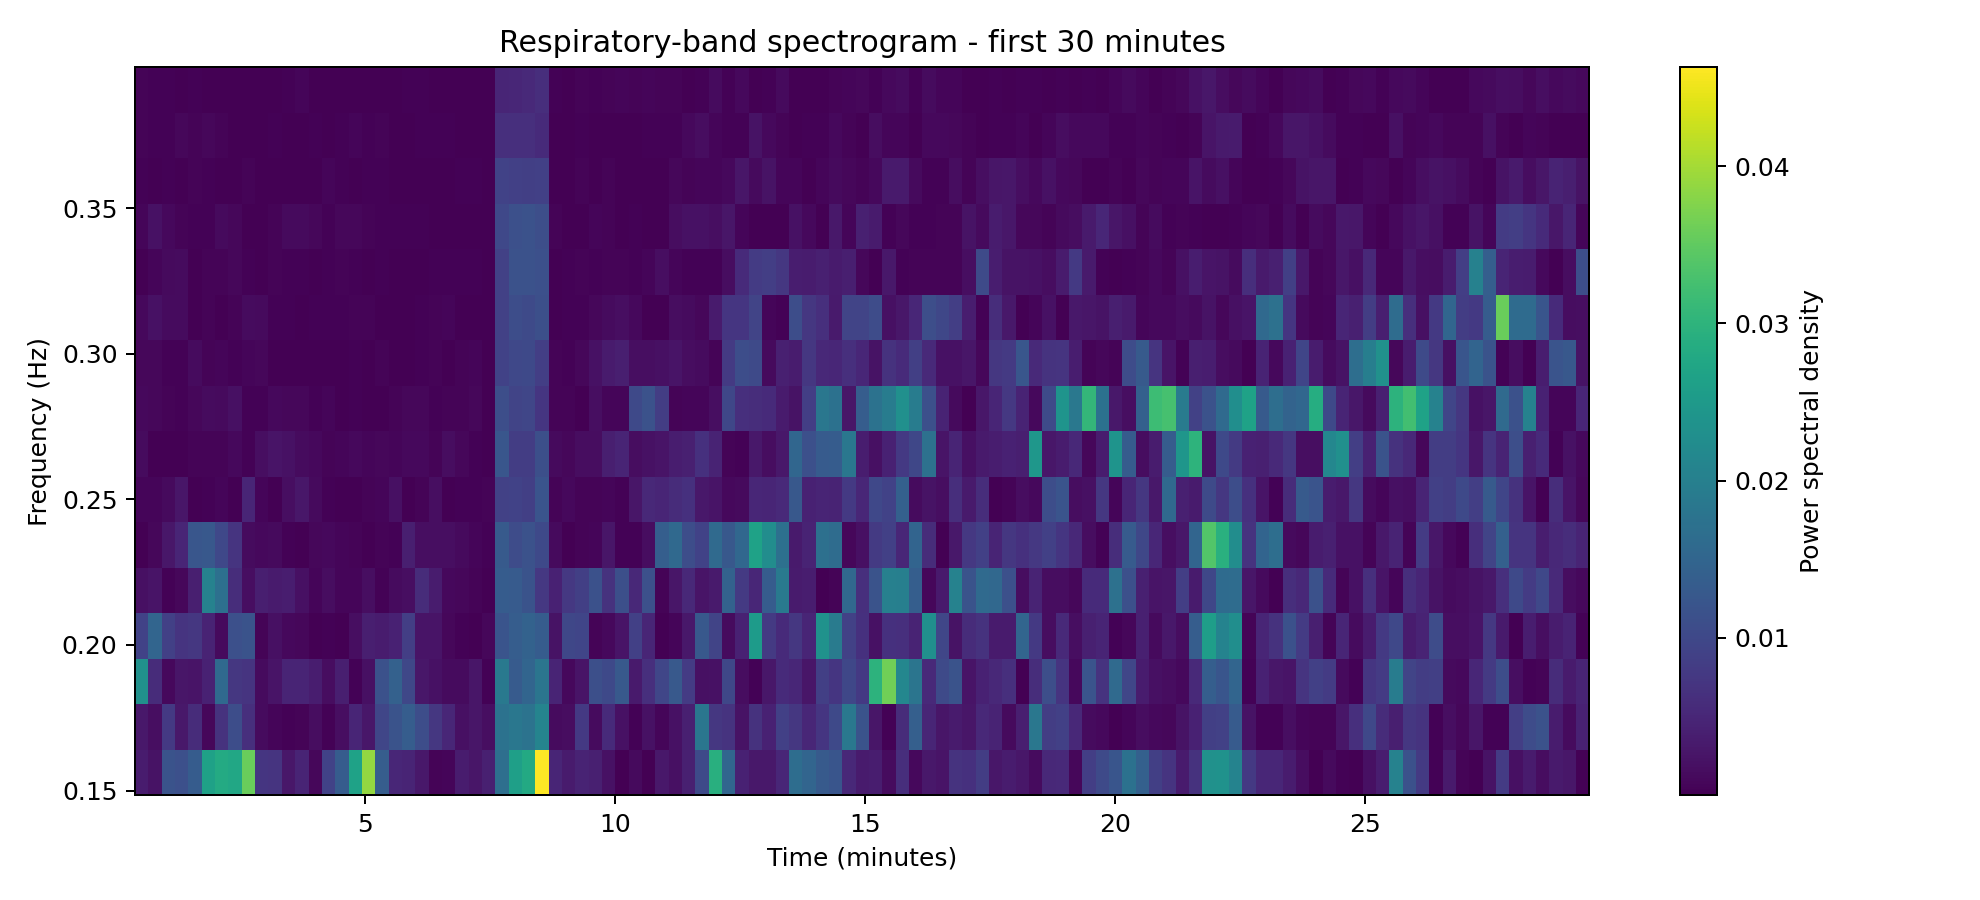
\includegraphics[width=0.90\linewidth]{respiratory_spectrogram_first30min.png}
    \caption{Respiratory-band spectrogram for the first 30 minutes. The
    location and strength of spectral components vary with time, rather than
    remaining at a single fixed frequency.}
    \label{fig:spectrogram}
\end{figure}

Together, the windowed estimates and spectrogram answer the stability question:
the ECG-derived respiratory-related frequency is clearly time-varying in this
record.

\section{Apnea-Related Exploratory Results}

The minute-level analysis contains 470 apnea-labelled minutes and only 19
normal-labelled minutes. The group summary is shown in
Table~\ref{tab:apneastats}.

\begin{table}[H]
\centering
\caption{Minute-level ECG-derived respiratory-rate estimates by apnea label.}
\label{tab:apneastats}
\begin{tabular}{lrrrrrr}
\toprule
Label & Count & Mean & Median & Std. dev. & Min & Max \\
      &       & \multicolumn{5}{c}{(breaths/min)} \\
\midrule
Normal (\texttt{N}) & 19  & 11.45 & 11.14 & 2.31 & 9.04 & 18.08 \\
Apnea (\texttt{A})  & 470 & 13.80 & 13.11 & 4.03 & 9.00 & 22.28 \\
\bottomrule
\end{tabular}
\end{table}

Figure~\ref{fig:boxapnea} shows the same comparison visually. In this record,
the apnea-labelled group has a higher median and a wider spread. The group
sizes are extremely different, so the result is descriptive rather than a
causal or clinical conclusion.

\begin{figure}[H]
    \centering
    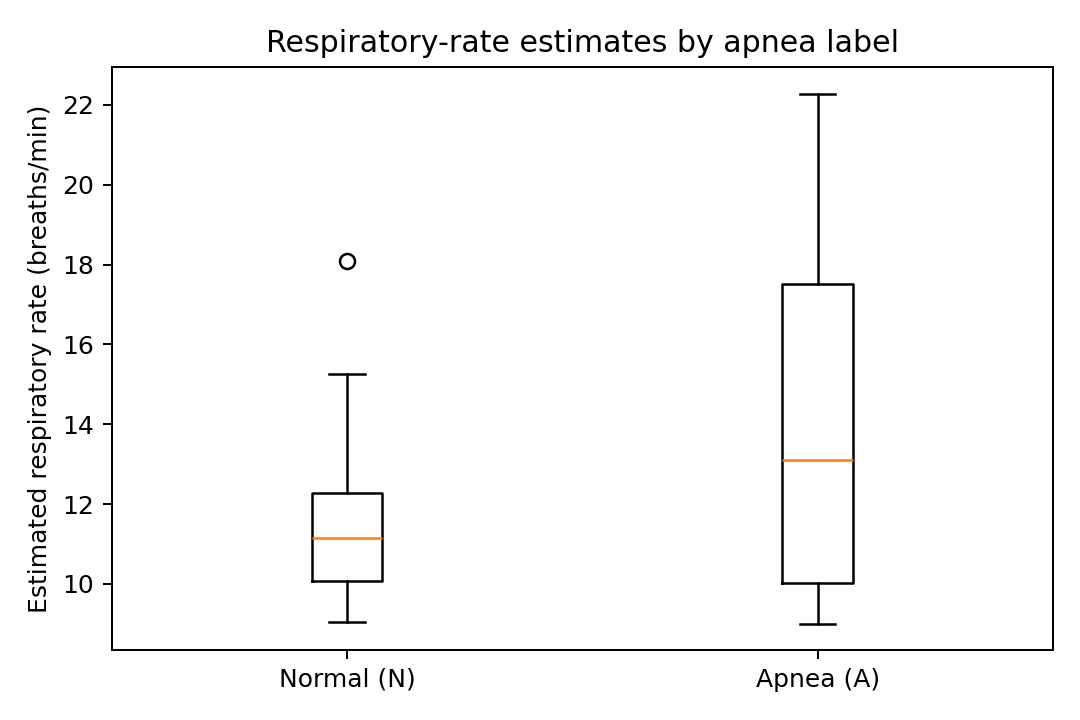
\includegraphics[width=0.60\linewidth]{normal_vs_apnea_resp_rate.png}
    \caption{Minute-level ECG-derived respiratory-rate estimates for normal and
    apnea-labelled intervals. The severe group-size imbalance is an important
    limitation of the comparison.}
    \label{fig:boxapnea}
\end{figure}

The exploratory logistic-regression model was evaluated on 98 test minutes:
94 labelled \texttt{A} and 4 labelled \texttt{N}. The confusion matrix in
Figure~\ref{fig:confusion} shows that three of four normal minutes and 83 of
94 apnea-labelled minutes were classified correctly.

\begin{figure}[H]
    \centering
    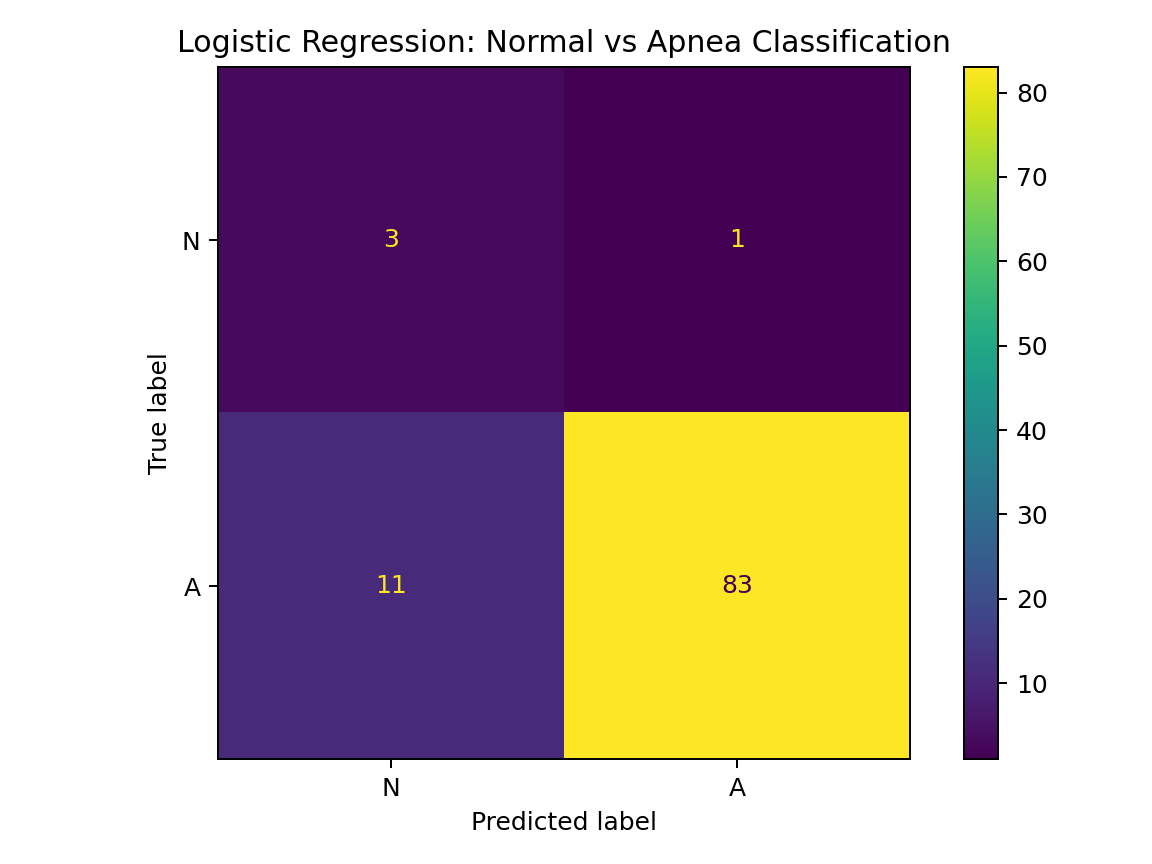
\includegraphics[width=0.62\linewidth]{apnea_confusion_matrix.png}
    \caption{Confusion matrix for the exploratory logistic-regression
    classifier. Rows are true labels and columns are predicted labels.}
    \label{fig:confusion}
\end{figure}

The overall test accuracy is 87.8\%. However, an always-\texttt{A} classifier
would obtain $94/98=95.9\%$ accuracy because the test set is highly imbalanced.
Accuracy alone is therefore misleading. The normal-class recall is 0.75, but it
is based on only four normal test samples; the normal-class precision is 0.21.
The classifier therefore demonstrates that the two simple features contain some
separative information within this record, but it is not a validated apnea
detector.

\chapter{Discussion}

\section{Main Findings in Relation to the Research Questions}

The first research question concerned whether a reliable long R--R interval
series could be constructed. The supplied QRS annotations matched the visible R peaks well in the ECG segment that was checked, and they were used to calculate 29,937 consecutive R--R intervals. This was sufficient for the current analysis, although using the supplied annotations instead of developing an independent R-peak detector is still a limitation.

The second research question was whether the R--R interval series contains useful respiratory-related information. The results suggest that the R--R interval series contains a reproducible respiratory-related spectral component. After processing the R--R series, clear frequency components were found within the 0.15--0.40 Hz range, and the first five-minute segment gave an estimated respiratory rate of 9.4 breaths/min. This is consistent with previous RSA-based studies
\citep{charlton2018,schaefer2008},
although the present estimates were not directly validated against a respiratory reference signal.

The third question concerned stability across time. The answer is clearly that
the estimate is not constant. Across 98 five-minute windows, values range from
9.38 to 19.69 breaths/min, with a mean of 13.58 and median of 12.19. The
spectrogram also shows that the frequency carrying stronger power changes over
time. This is an important result because it prevents over-interpreting one
short segment as representative of the full 8.21-hour recording.

The fourth question asked whether respiratory-related ECG behaviour differs
between normal and apnea-labelled periods. In record \texttt{a01}, the
apnea-labelled minutes have a higher median estimate (13.11 breaths/min) and a
larger spread than the normal-labelled minutes (median 11.14 breaths/min).
However, only 19 normal minutes are available compared with 470 apnea-labelled
minutes, so this finding is exploratory.

\section{Method Refinement, Self-Learning and Problem Solving}

Some parts of the method were changed during the project after checking how the data behaved. These changes were made based on the results of the analysis rather than simply following the original plan.

First, the initial project plan placed more emphasis on developing an
independent R-peak detector. However, the supplied QRS annotations showed good agreement with the visible R peaks and were already available for the record. The project scope was therefore adjusted to focus more on extracting respiratory-related information from the R--R interval series. This allowed the analysis to concentrate on developing one complete and interpretable workflow rather than several partially developed methods.

Second, the respiratory search range needed to be chosen carefully. Early spectra showed strong low-frequency power near the lower end of wider search ranges. Instead of simply choosing the largest peak in the spectrum, the final method uses the literature-supported 0.15--0.40 Hz HRV high-frequency range \citep{taskforce1996}. The result from the first five-minute window is still close to the lower boundary, so the wider spectrum is also shown. This makes it clear that the estimated respiratory rate can depend on the chosen frequency range.

Third, the R--R data are not sampled at regular time intervals. The data were therefore interpolated to 4 Hz before Welch analysis. The interpolated curve was then compared with the original R--R samples to check that the main pattern had not changed noticeably. This provides a simple visual check that the interpolation was suitable for the later frequency analysis.

Fourth, an incomplete ECG download during development showed the need for a data-integrity check. The number of samples in the ECG file was therefore compared with the expected sample count given in the header. This is a simple check, but it helps make the analysis more reliable and reproducible because an incomplete file may still be read successfully while containing less data than expected.

Finally, the classification results show that accuracy alone can be misleading when the classes are highly imbalanced. Although the model achieved an accuracy of 87.8\%, 94 of the 98 test samples belonged to class \texttt{A}. A model that simply predicts \texttt{A} for every sample would therefore also achieve a high accuracy. For this reason, the confusion matrix, precision and recall for each class, and the class imbalance should also be considered when evaluating the classifier.

\section{Reliability of the Respiratory Estimate}

The estimated respiratory rate should be interpreted carefully because breathing is not measured directly. Instead, the method finds the strongest frequency component in the R--R interval series within the selected frequency range and converts this frequency into breaths per minute.

The first five-minute spectrum demonstrates this limitation directly: a strong
component is visible below 0.15 Hz, while the selected peak at 0.156 Hz lies
close to the band boundary. The conventional HRV high-frequency band provides
a defensible starting point \citep{taskforce1996}, but it does not guarantee
that true respiration always lies inside the range. The output is therefore
best described as an ECG-derived respiratory-related estimate.

The choice of Welch segment length also matters. With 256 samples at 4 Hz,
adjacent frequency bins are separated by 0.015625 Hz, or about
0.94 breaths/min. A longer segment would improve nominal frequency resolution
but reduce the amount of averaging available within short windows. The chosen
value is therefore a compromise rather than a uniquely correct parameter.

The direct waveform exploration also supports a cautious interpretation. The
30-minute ECG standard deviations are fairly stable, but the full-record
amplitude range is wider than the first 10 seconds. Short artefacts or
morphology changes can still influence QRS timing and R--R variability even
when long-block statistics appear stable.

\section{Limitations and Scope}

The most important limitation is that the available reference respiratory signals for record \texttt{a01} were not included in the present analysis. Therefore, the ECG-derived estimates were not directly compared with a respiratory reference rate. The spectral peak selected from the R--R interval series cannot be treated as a validated breathing-rate measurement. Instead, the results are evaluated using internal consistency, behaviour across different time windows, physiological plausibility, and previous evidence that respiration can modulate R--R intervals.

The detailed analysis in this report focuses mainly on record \texttt{a01}. Although the original plan included comparisons across several records, the final report focuses on a more detailed and reproducible analysis of this single record. This allows the analysis to be explained more clearly, but the results cannot be assumed to apply to other subjects.

The supplied QRS annotations are used as timing references instead of an
independently developed detector. R--R variability is influenced by factors
other than respiration, the search-band and Welch parameters affect the output,
and the apnea labels are severely imbalanced. The exploratory classifier is
trained and tested on minutes from the same record, so neighbouring windows are
not independent in the same way as data from different subjects.

For these reasons, the project should not be interpreted as a clinical
respiratory monitor or apnea diagnostic system. Its contribution is a
transparent and reproducible demonstration of how respiratory-related
information can be extracted from ECG-derived R--R timing, together with an
explicit analysis of where that interpretation becomes uncertain.

\chapter{Conclusion}

A complete ECG-to-respiratory analysis pipeline was developed for PhysioNet
Apnea-ECG record \texttt{a01}. The ECG was read and scaled from WFDB metadata,
basic data integrity was checked, waveform variability was explored directly,
and supplied QRS annotations were compared with visible R peaks before being
used. These timings produced 29,937 R--R intervals from 29,938 QRS annotations.

After broad outlier screening, the irregular R--R series was interpolated to
4 Hz, detrended and analysed using Welch's power spectral density estimate.
The first five-minute interval produced a dominant in-band frequency of
0.156 Hz, equivalent to 9.4 breaths/min. Across 98 five-minute windows, the
estimates ranged from 9.38 to 19.69 breaths/min. The full-window plot and the
30-minute spectrogram both show that the respiratory-related spectral behaviour
changes with time.

The apnea-related analyses were useful extensions rather than the centre of the project. Apnea-labelled minutes showed a different distribution of ECG-derived respiratory-rate estimates, and a logistic-regression model with balanced class weights was explored as a simple classification extension. However, the extreme class imbalance, single-record design and lack of direct respiratory-reference validation prevent strong diagnostic conclusions.

Therefore, the main achievement of this project is not a single respiratory rate value, but a repeatable workflow for extracting time-varying respiratory-related spectral information from the R-R interval derived from the electrocardiogram. The results show that the proposed method can consistently produce in-band estimates across the recording. However, these estimates were not directly validated against a respiratory reference signal and should not be interpreted as direct measurements of breathing rate. Future work could compare the ECG-derived estimates with the available respiratory signals and evaluate the method across additional records.

\begin{appendices}
\chapter{Reproducibility Notes}

The core analysis is reproduced from the project root using

\begin{verbatim}
.\.venv\Scripts\python.exe run_analysis.py --no-download
\end{verbatim}

and the exploratory classifier using

\begin{verbatim}
.\.venv\Scripts\python.exe apnea_classification.py
\end{verbatim}

The report figures are generated from the project analysis and stored in
the \texttt{figures} directory. The five-minute and minute-level result tables
are stored in \texttt{results/respiratory\_rate\_5min\_windows.csv} and
\texttt{results/respiratory\_rate\_by\_apnea\_minute.csv}. The additional
summary figures used to discuss robustness are generated directly from these
results and from the raw ECG samples. All numerical values reported in the
Results chapter can therefore be recreated from the supplied data and code.
\end{appendices}

\clearpage
\addcontentsline{toc}{chapter}{References}
\begin{thebibliography}{99}

\bibitem[Charlton et al.(2018)]{charlton2018}
P. H. Charlton et al., ``Breathing Rate Estimation From the Electrocardiogram and Photoplethysmogram: A Review,'' \textit{IEEE Reviews in Biomedical Engineering}, vol. 11, pp. 2--20, 2018. doi: 10.1109/RBME.2017.2763681.

\bibitem[Sch\"afer and Kratky(2008)]{schaefer2008}
A. Sch\"afer and K. W. Kratky, ``Estimation of breathing rate from respiratory sinus arrhythmia: comparison of various methods,'' \textit{Annals of Biomedical Engineering}, vol. 36, no. 3, pp. 476--485, 2008. doi: 10.1007/s10439-007-9428-1.

\bibitem[Task Force(1996)]{taskforce1996}
Task Force of the European Society of Cardiology and the North American Society of Pacing and Electrophysiology, ``Heart rate variability: standards of measurement, physiological interpretation and clinical use,'' \textit{Circulation}, vol. 93, no. 5, pp. 1043--1065, 1996. doi: 10.1161/01.CIR.93.5.1043.

\bibitem[Welch(1967)]{welch1967}
P. D. Welch, ``The use of fast Fourier transform for the estimation of power spectra: A method based on time averaging over short, modified periodograms,'' \textit{IEEE Transactions on Audio and Electroacoustics}, vol. 15, no. 2, pp. 70--73, 1967. doi: 10.1109/TAU.1967.1161901.

\bibitem[Penzel et al.(2000)]{penzel2000}
T. Penzel, G. B. Moody, R. G. Mark, A. L. Goldberger, and J. H. Peter, ``The Apnea-ECG Database,'' \textit{Computers in Cardiology}, vol. 27, pp. 255--258, 2000. doi: 10.1109/CIC.2000.898505.

\bibitem[Goldberger et al.(2000)]{goldberger2000}
A. L. Goldberger et al., ``PhysioBank, PhysioToolkit, and PhysioNet: Components of a New Research Resource for Complex Physiologic Signals,'' \textit{Circulation}, vol. 101, no. 23, pp. e215--e220, 2000. doi: 10.1161/01.CIR.101.23.e215.

\bibitem[Weinstein et al.(2026)]{weinstein2026}
A. Weinstein, J. Rodi\~no, and M. Otero, ``Effects of electrocardiogram QRS detection algorithms in heart rate variability metrics,'' \textit{Scientific Reports}, vol. 16, article 18589, 2026. doi: 10.1038/s41598-026-49215-6.

\bibitem[Penzel et al.(2002)]{penzel2002}
T. Penzel, J. McNames, P. de Chazal, B. Raymond, A. Murray, and G. Moody, ``Systematic comparison of different algorithms for apnoea detection based on electrocardiogram recordings,'' \textit{Medical \& Biological Engineering \& Computing}, vol. 40, no. 4, pp. 402--407, 2002. doi: 10.1007/BF02345072.

\bibitem[de Chazal et al.(2003)]{dechazal2003}
P. de Chazal, C. Heneghan, E. Sheridan, R. Reilly, P. Nolan, and M. O'Malley, ``Automated processing of the single-lead electrocardiogram for the detection of obstructive sleep apnoea,'' \textit{IEEE Transactions on Biomedical Engineering}, vol. 50, no. 6, pp. 686--696, 2003. doi: 10.1109/TBME.2003.812203.

\bibitem[de Chazal et al.(2004)]{dechazal2004}
P. de Chazal, T. Penzel, and C. Heneghan, ``Automated detection of obstructive sleep apnoea at different time scales using the electrocardiogram,'' \textit{Physiological Measurement}, vol. 25, no. 4, pp. 967--983, 2004. doi: 10.1088/0967-3334/25/4/015.

\bibitem[Roche et al.(2003)]{roche2003}
F. Roche et al., ``Predicting sleep apnoea syndrome from heart period: a time-frequency wavelet analysis,'' \textit{European Respiratory Journal}, vol. 22, no. 6, pp. 937--942, 2003. doi: 10.1183/09031936.03.00104902.



\end{thebibliography}

\end{document}
